\documentclass[border=1pt]{standalone}
\usepackage[dvipsnames]{xcolor}
\usepackage{tikz}                       % Graphen und kommutative Diagramme
\usetikzlibrary{patterns}               % Um schraffierte Formen in der tikzpicture-Umgebung zu zeichnen.

\newcommand{\ul}[1]{\underline{\smash{#1}}}
\begin{document}
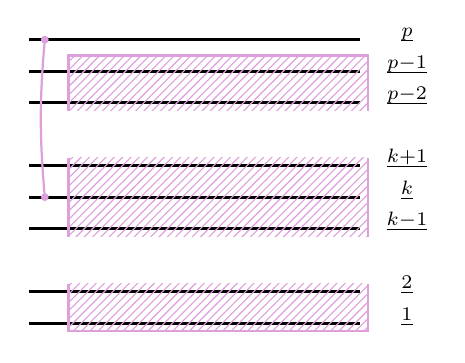
\begin{tikzpicture}[scale=.4, line width=1pt]
    % Linien.
    \foreach \i in {0,1,3,4,5,7,8,9}
    {
        \draw[color=black] (-.5,\i) -- (10,\i);   
    }
    
    % Beschriftung der Linien.
    \draw node at (11.5,0) {$\scriptstyle \ul1$};
    \draw node at (11.5,1) {$\scriptstyle \ul2$};
    \draw node at (11.5,3) {$\scriptstyle \ul{k-1}$};
    \draw node at (11.5,4) {$\scriptstyle \ul k$};
    \draw node at (11.5,5) {$\scriptstyle \ul{k+1}$};
    \draw node at (11.5,7) {$\scriptstyle \ul{p-2}$};
    \draw node at (11.5,8) {$\scriptstyle \ul{p-1}$};
    \draw node at (11.5,9) {$\scriptstyle \ul p$};
    
    
    % Grüne Blöcke.
    \fill[pattern=north east lines, pattern color=Plum] (1 - .25, 0 - .25) -- (10 + .25, 0 - .25) -- (10 + .25, 1 + .25) -- (1 - .25, 1 + .25) -- cycle;
    \fill[pattern=north east lines, pattern color=Plum] (1 - .25, 3 - .25) -- (10 + .25, 3 - .25) -- (10 + .25, 5 + .25) -- (1 - .25, 5 + .25) -- cycle;
    \fill[pattern=north east lines, pattern color=Plum] (1 - .25, 7 - .25) -- (10 + .25, 7 - .25) -- (10 + .25, 8 +  .5) -- (1 - .25, 8 +  .5) -- cycle;
    
    % Berandung der grünen Blöcke.
    \draw[color=Plum, thick] (1 - .25, 1 + .25) -- (1 - .25, 0 -.25) -- ( 10 + .25, 0 - .25) -- (10 + .25, 1 + .25);
    \draw[color=Plum, thick] (1 - .25, 5 + .25) -- (1 - .25, 3 -.25);
    \draw[color=Plum, thick] (10 + .25, 5 + .25) -- (10 + .25, 3 -.25);
    \draw[color=Plum, thick] (1 - .25, 7 - .25) -- (1 - .25, 8 +  .5) -- (10 + .25, 8 +  .5) -- (10 + .25, 7 - .25);
    
    % Transposition.
    \draw node[inner sep=1pt, fill=Plum, shape=circle] at (0, 4) {};
    \draw node[inner sep=1pt, fill=Plum, shape=circle] at (0, 9) {};
    \draw[color=Plum, thick] (0, 4) to[in=265, out=95] (0, 9);
\end{tikzpicture}
\end{document}